\documentclass{article}

\usepackage[frenchb]{babel}
\usepackage[T1]{fontenc}
\usepackage[utf8]{inputenc}
\usepackage{graphicx}

\title{Manuel d'utilisation de l'application ToDoList}
\author{Anthony Brunel et Antoine Laurent}

\date{\today}

\begin{document}
\maketitle
\newpage
\tableofcontents
\listoffigures
\newpage

\section{Lancement de l'application}
Pour lancer l'application, il suffit de double cliquer sur ToDoList.jar, de compiler les sources en incluant le librairie JCalendar ou bien sous Linux via la commande : \verb+java -jar ToDoList.jar+
\newline
\newline
Une fois l'application lancée vous arriverez sur la fenêtre principale (Figure~\ref{Fenêtre principale}), c'est à partir de cette fenêtre que vous allez gérer vos tâches. 
\newline
Si vous souhaitez quitter l'application il faudra cliquer sur la croix rouge ou bien utiliser la combinaison de touche Alt + f4. Vos modification seront automatiquement sauvegarde dans le fichier sauvegarde.todo.

\begin{figure}[h]
	\centering
	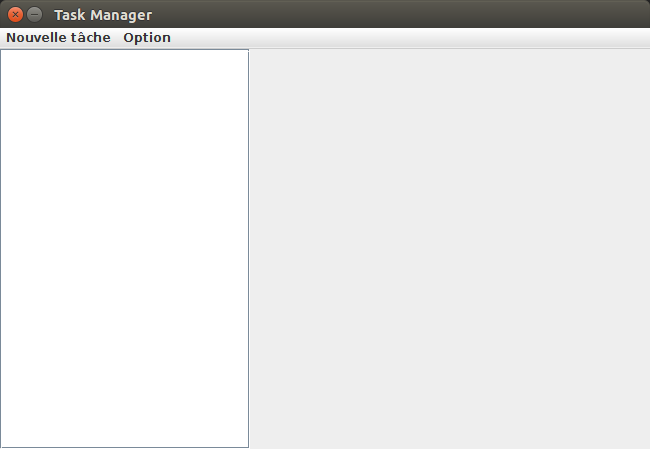
\includegraphics[scale=0.34]{images/MainDIsplay.png}
	\caption{Fenêtre principale}
	\label{Fenêtre principale}
\end{figure}

%\clearpage
\section{Les actions possibles}
Lors de la première utilisation, lorsque vous êtes sur la fenêtre principale plusieurs options s'offre alors à vous:
\newline

\begin{itemize}
	\item Créer une tâche au long cours.
	\item Créer une tâche ponctuelle.
	\item Créer, modifier ou supprimer une catégorie.
	\item Générer le bilan.
	\item Effectuer des tris sur nos tâches.
\end{itemize}

\subsection{Créer une tâche}
Pour créer une tâche il faut appuyer sur le bouton "Nouvelle tâche" dans le menu (Figure~\ref{Taches barre}), ensuite vous pourrez choisir entre une tâche au long cours ou une tâche ponctuelle.

\begin{figure}
	\centering
	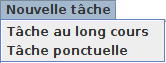
\includegraphics[scale=0.8]{images/MenuTache.png}
	\caption{Ajout d'une tâche}
	\label{Taches barre}
\end{figure}

Une fois choisie il ne reste plus qu'à entrer les informations de votre tâche (Figures \ref{Tâche au long cours} et \ref{Tâche Ponctuelle}). Il faut appuyer sur "Valider" pour valider la tâche.

\begin{figure}[!ht]
	\centering
	\begin{minipage}[t]{5cm}
		\centering
		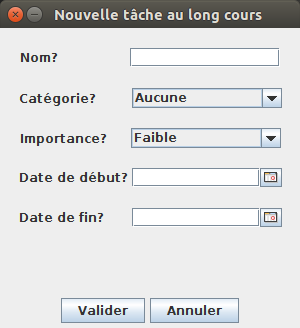
\includegraphics [scale=0.34]{images/NewTAsk1.png}
		\caption{Tâche au long cours}
		\label{Tâche au long cours}
	\end{minipage}
	\begin{minipage}[t]{5cm}
		\centering
		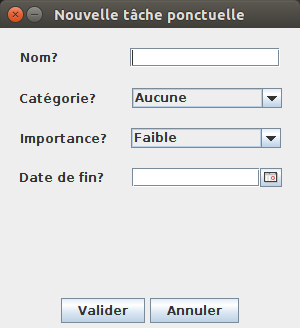
\includegraphics [scale=0.34]{images/NewTAsk2.png}
		\caption {Tâche Ponctuelle}
		\label{Tâche Ponctuelle}
	\end{minipage}
\end{figure}

\textbf{NB :} Vous pouvez soit rentrer les dates au clavier sous le format jj/MM/aaaa ou les choisir avec le calendrier.
\newline
\par
Lorsque vous ajoutez une tâche, vous retournerez sur la fenêtre principale, les tâches au long cours apparaîtront bleues et les tâches ponctuelles vertes. Le nombre de jours restant avant la fin de la tâche sera indiqué à côté de celle-ci.
De plus, si une tâche est en retard un petit panneau rouge vous l'indiquera.
Pour modifier les paramètres d'une tâche il vous faudra la sélectionner dans la liste située à gauche enfin sur la droite s'affichera les informations de cette tâche. Vous pourrez la modifier en cliquant sur le bouton Modifier vous pourrez ensuite "Valider" vos modification ou les "Annuler". Le bouton Supprimer permet d'éffacer intégralement une tâche, si vous souhaité finir une tâche vous avez deux possibilités soit en cliquant sur Tâche finie pour les tâches ponctuelle soit en modifiant la tâche et en faisant avancer l'évolution de celle-ci à 100% Une tâche terminée est sauvegardée en mémoire contrairement à une tâche que vous supprimez.
(Figure \ref{Fenetre principale 2}).

\begin{figure}[!h]
	\centering
	\includegraphics[scale=0.34]{images/CaptureMainDIsplay3.png}
	\caption{Fenetre Principale avec tâches}
	\label{Fenetre principale 2}
\end{figure}

\clearpage
\subsection{Créer Modifier une catégoire}
Pour accéder au paramètre des catégories il vous suffira de cliquer sur "Option" puis "Catégorie" (Figure \ref{barre Opiton}).

\begin{figure}[h]
	\centering
	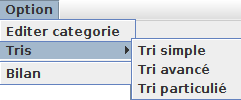
\includegraphics[scale=0.6]{images/MenuOption.png}
	\caption{Menu Option}
	\label{barre Opiton}
\end{figure}

Ensuite vous pourrez créer de nouvelle catégorie ou bien les modifier et les supprimer. La catégorie Aucune est une catégorie par défaut vous ne pouvez pas la modifier ni la supprimer. (Figure \ref{modif Opiton}).

\begin{figure}[h]
	\centering
	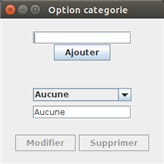
\includegraphics[scale=0.8]{images/Capture_edit_categorie.jpg}
	\caption{Modification d'une Catégorie}
	\label{modif Opiton}
\end{figure}

%\clearpage
\subsection{Générer le bilan}

Notre application permet aussi de générer le bilan, pour ceci il faut cliquer sur le bouton "Option" puis "Bilan" (Figure \ref{barre Opiton}).
Une nouvelle fenêtre s'ouvrira où il faudra rentrer la date de début et la date de fin de la période sur laquelle vous souhaitez générer le bilan puis cliquer sur "Générer" (Figrue \ref{bilan}).

\begin{figure}
	\centering
	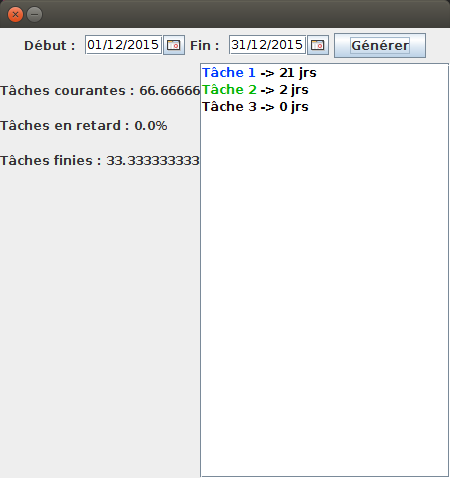
\includegraphics[scale=0.5]{images/CaptureDisplayBilan.png}
	\caption{Fenêtre bilan}
	\label{bilan}
\end{figure}

La fenêtre contiendra les tâches comprise dans le bilan, leur statut (les tâches finies sont en noir les autres sont de la couleur de leur type), et le pourcentage de tâches courantes, en retard et finies sur cette période.

\subsection{Les tris}

Il y a trois tris à disposition, le tri simple qui tri par ordre de proximité
d'échéance croissante pour les tâches dont l'échéance n'est pas échue, et décroissante
pour les tâches dont l'échéance est échue, le tri avancé (tris en fonction des échéances intermédiaires des tâche au long cours) et le tri par importance qui présente 9 tâches : une importante, 3 moyennes, et 5 faible. Pour les activer il faut cliquer sur "Option" puis cliquer le tri souhaité. Attention si vous souhaitez re-afficher l'ensemble des tâches il sufira de cliquer sur le tri simple ou le tri avancé.(Figure \ref{barre Opiton}).

\end{document}
